\documentclass{article}
\usepackage{graphicx} % Required for inserting images

\title{EECS510 Arithmetic Language Automaton}
\author{Jake Kice}
\date{November 2024}

\usepackage{tikz}
\usetikzlibrary{automata, positioning, arrows.meta, calc}
\tikzset{
->, node distance=3cm,
>={Latex[width=3mm,length=3mm]},
every  edge/.append style={thick, scale=1.8},
every state/.style={thick},
every  node/.append style={scale=1.4},
initial text=$ $, }

\tikzstyle{accepting}=[path picture={%
        \draw let
                \p1 = (path picture bounding box.east),
                \p2 = (path picture bounding box.center)
                in
                        (\p2) circle (\x1 - \x2 - 2pt); % adjust `2pt` here for clarity
}]

\begin{document}

\maketitle

%\section{Introduction}

    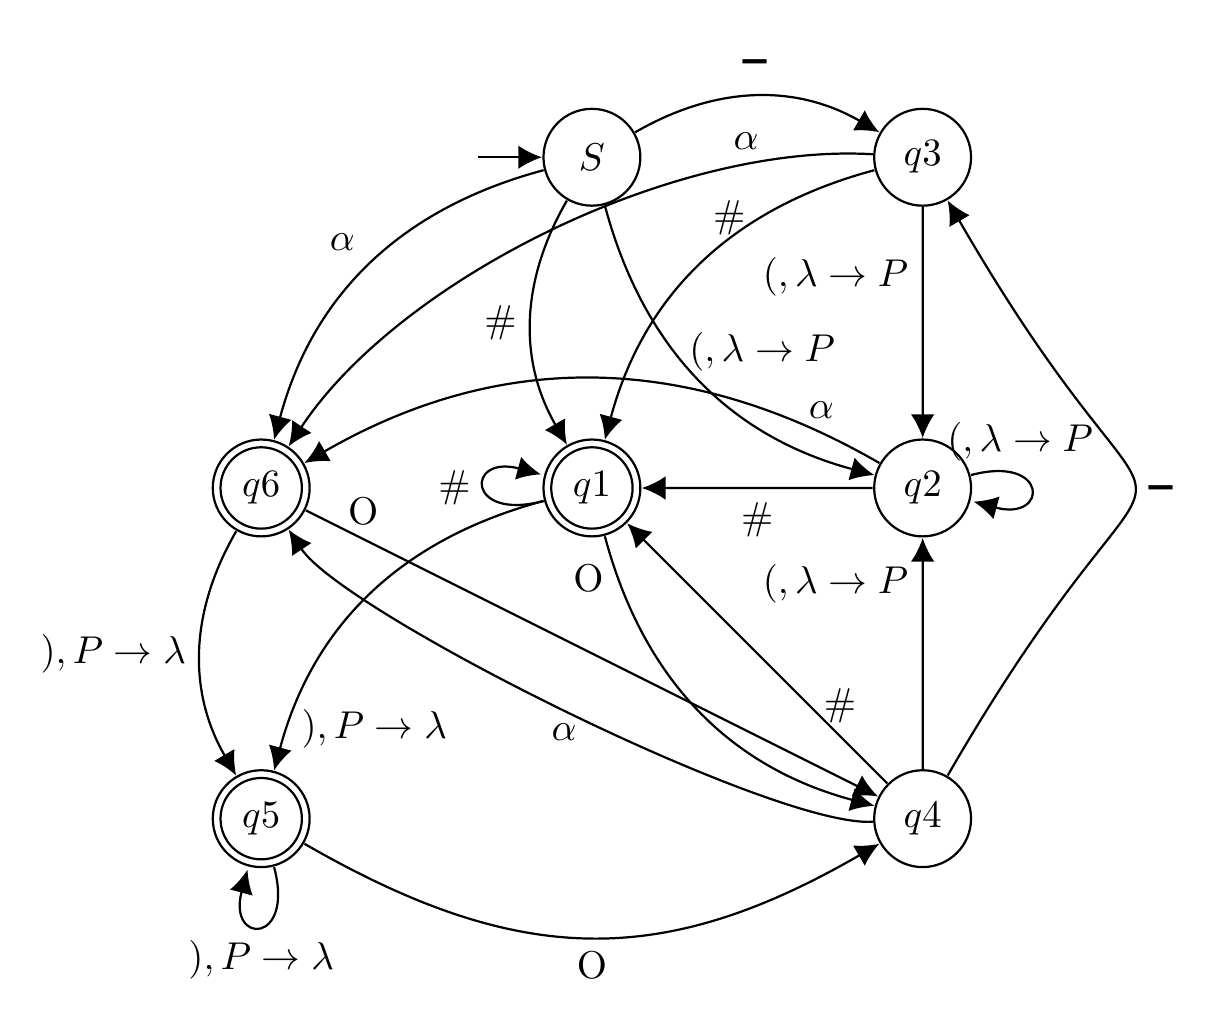
\begin{tikzpicture}
            \node[state,initial] (S) {$S$};
            \node[state, accepting, below of=S] (1) {$q1$};
            \node[state, accepting, left of=1] (6) {$q6$};
            \node[state, right of=1] (2) {$q2$};
            \node[state, right of=S] (3) {$q3$};
            \node[state, below of=2] (4) {$q4$};
            \node[state, accepting, below of=6] (5) {$q5$};

            % Transitions from S
            \draw (S) edge[bend right, left] node{$\#$} (1);
            \draw (S) edge[bend right, right] node[pos=.4]{$(,\lambda\rightarrow P$} (2);
            \draw (S) edge[bend left, above] node{\Huge -} (3);
            \draw (S) edge[bend right, above left] node{$\alpha$} (6);

            % Transitions from 1
            \draw (1) edge[loop left] node{\#} (1);
            \draw (1) edge[bend right, left] node[pos=.1]{O} (4);
            \draw (1) edge[bend right, right] node[pos=.9]{$),P\rightarrow\lambda$} (5);

            % Transitions from 2
            \draw (2) edge[below] node{$\#$} (1);
            \draw (2) edge[loop right, above] node[pos=.3]{$(,\lambda\rightarrow P$} (2);
            \draw (2) edge[bend right, above] node[pos=.1]{$\alpha$} (6);

            % Transitions from 3
            \draw (3) edge[bend right, left] node[pos=.3]{$\#$} (1);
            \draw (3) edge[left] node[pos=.3]{$(,\lambda\rightarrow P$} (2);
            \draw (3) edge[bend right, distance=40, above] node[pos=.2]{$\alpha$} (6);

            % Transitions from 4
            \draw (4) edge[right] node[pos=.3]{$\#$} (1);
            \draw (4) edge[left] node[pos=.8]{$(,\lambda\rightarrow P$} (2);
            \draw (4) edge[bend right, distance=100, right] node[pos=.5]{\Huge -} (3);
            \draw (4) edge[bend left, distance=20, below] node{$\alpha$} (6);

            % Transitions from 5
            \draw (5) edge[bend right, distance=50, below] node{O} (4);
            \draw (5) edge[loop below] node{$),P\rightarrow\lambda$} (5);

            % Transitions from 6
            \draw (6) edge[above] node[pos=.1]{O} (4);
            \draw (6) edge[bend right, left] node{$),P\rightarrow\lambda$} (5);
            
     \end{tikzpicture}

    $\alpha=\{a,b,...z\}$ \newline
    $\#=\{0,1,...9\}$ \newline
    $O=\{+,-,*,/,\%,\wedge\}$ \newline
    Note: all transitions other than left paren and right paren are stack agnostic (they ignore the stack). As such, all transitions in the diagram that do not show stack interaction can be considered as $s, \lambda \rightarrow \lambda$, where s is the input symbol.
    
\end{document}
